\documentclass[10pt]{beamer}

\usetheme{metropolis}
\usepackage{appendixnumberbeamer}

\usepackage{booktabs}
\usepackage[scale=2]{ccicons}

\usepackage{pgfplots}
\usepgfplotslibrary{dateplot}

\usepackage{xspace}
\newcommand{\themename}{\textbf{\textsc{metropolis}}\xspace}

\usepackage{float}
\usepackage{subcaption}
\usepackage{epstopdf}

\usepackage{mathtools}
\newcommand{\conv}{\mathop{\bf conv}}
\usepackage{bm}

\usepackage{amsmath,amssymb}
\usepackage{amsthm}
% \newtheorem{theorem}{Theorem}

% \usepackage{marvosym}

% \let\theorem\relax
% \newtheorem{proposition}{Proposition}
% \newtheorem{definition}{Definition}
% \newtheorem{corollary}{Corollary}
% \newcommand\numberthis{\addtocounter{equation}{1}\tag{\theequation}}
% \DeclareMathOperator{\sign}{\text{sgn}}
% \DeclareMathOperator*{\argmin}{arg\,min}
% \DeclareMathOperator{\intr}{int}
% \DeclareMathOperator{\dom}{dom}
% \DeclareMathOperator{\rot}{\text{rot}}

\usepackage{tikz}
\usetikzlibrary{scopes}
\usetikzlibrary{shapes.misc}
\usetikzlibrary{shapes.arrows}
\tikzset{cross/.style={cross out, draw=black, minimum size=2*(#1-\pgflinewidth), inner sep=0pt, outer sep=0pt}, %default radius will be 1pt. 
cross/.default={2pt}}

\title{Exact Bounds on the Contact Driven Motion of a Sliding Object}
\subtitle{With Applications to Robotic Pulling}
\date{\today}
\author{Eric Huang$^1$, Ankit Bhatia$^2$, Byron Boots$^1$, Matt Mason$^2$}
\institute{$^1$Georgia Institute of Technology, $^2$Carnegie Mellon University}
% \titlegraphic{\hfill\includegraphics[height=1.5cm]{logo.pdf}}

\begin{document}

\maketitle

\begin{frame}{Table of contents}
  \setbeamertemplate{section in toc}[sections numbered]
  \tableofcontents[hideallsubsections]
\end{frame}

\section{Introduction}

\begin{frame}{Introduction}
  Hello
\end{frame}

\section{Background}

\begin{frame}{Quasi-static Theory of Planar Pushing}
  % Theory
  \begin{columns}[c,onlytextwidth]
    \column{0.5\textwidth}

    \begin{list}{}{
        \setlength{\leftmargin}{0pt}
        \setlength{\labelwidth}{0pt}
        \setlength{\labelsep}{0pt}
      }
    \item%\<1->%\ 
      Twist: 
      \begin{equation*}
        \mathbf{v}^+ = [\mathbf{v}^T, \omega]^T
      \end{equation*}
    \item%<2-> 
      Body point velocity:
      \begin{equation*}
        A(\mathbf{x})\mathbf{v}^+ = 
        \begin{bmatrix*}[r]
          1 & 0 & -x_2 \\
          0 & 1 &  x_1
        \end{bmatrix*}\mathbf{v}^+
      \end{equation*}
    \item%<3-> 
      Total frictional moment:
      \begin{equation*}
        \mathbf{m}_f = -\mu\int_{R}\mathbf{r}\times\frac{A(\mathbf{r})\mathbf{v}^+}{\lVert A(\mathbf{r})\mathbf{v}^+ \rVert} p(\mathbf{r}) dA
      \end{equation*}
    \item%<4-> 
      Quasi-static assumption:
      \begin{equation*}
        \mathbf{m}_f = 0
      \end{equation*}
    \end{list}

    \column{0.5\textwidth}
    \begin{figure}
      \centering
      \def\iangle{35} % Angle of the inclined plane
      \begin{tikzpicture}[
        scale=1.25, every node/.style={scale=1.25},
        force/.style={>=latex,draw=black,fill=black},
        axis/.style={densely dashed,draw=gray,font=\small},
        ]
        \fill[draw=black,fill=blue!10,thin,rotate=\iangle] (-0.3,-0.5) rectangle (2.3,.5);
        \draw[rotate=\iangle] (1,0) circle[radius=2.4pt] node[cross] {};
        \draw[rotate=\iangle] (1,0) node[above right] {\tiny CoP};
        \draw [->,line width=1pt,rotate=-62.5] (0,0) ++(0,1) arc (90:30:1.0) node[right] {$\omega$};
        {[axis,->]
          \draw (0,0) -- (2.5,0) node[right] {$x$};
          \draw (0,0) -- (0,2.5) node[above] {$y$};
        }
        {[force,->]
          \draw (0,0) -- ++(0,1.5) node[right] {$\mathbf{v}$};
        }
        \fill (0,0) circle [radius=1.pt];
        % \fill (1.2207,0) circle [radius=1.pt] node[below right] {$x_{\text{\tiny IC}}$};

      \end{tikzpicture}
      % \caption{Motion of a press-pulled slider.}
      % \BB{Define variables and provide a short explanation of the figure.}}
      % \label{fig:presspull-motion}
    \end{figure}

  \end{columns}
\end{frame}

\begin{frame}{Moment Envelope}
  \begin{columns}[c,onlytextwidth]
    \column{0.5\textwidth}
    % Given twist $\mathbf{v}^+$, region $R$ \textbf{(a)}
    \begin{itemize}%[<+->]
      \item[\textbf{(a)}] Given twist $\mathbf{v}^+$, region $R$
      \item[\textbf{(b)}] Torque from unit pressure at $\mathbf{r}$:
      \begin{equation*}
        g(\mathbf{r}) = -\mu\,\mathbf{r}\times \frac{A(\mathbf{r})\mathbf{v}^+}{\lVert A(\mathbf{r})\mathbf{v}^+ \rVert}
      \end{equation*}
      Moment surface function:
      \begin{equation*}
        G(\mathbf{r}) =
        \begin{bmatrix*}
          \mathbf{r}\\
          g(\mathbf{r})
        \end{bmatrix*}
      \end{equation*}
    \item[\textbf{(c)}] Moment envelope:
      \begin{equation*}
        \conv G(R)
      \end{equation*}
    \item[\textbf{(d)}] Feasible CoPs ($\mathbf{m}_f=0$):
      \begin{equation*}\conv G(R) \cap \{z=0\}\end{equation*}
    \end{itemize}

    \column{0.5\textwidth}
    \begin{figure}[t]
      \centering
      \begin{subfigure}[b]{0.49\textwidth}
        \centering
        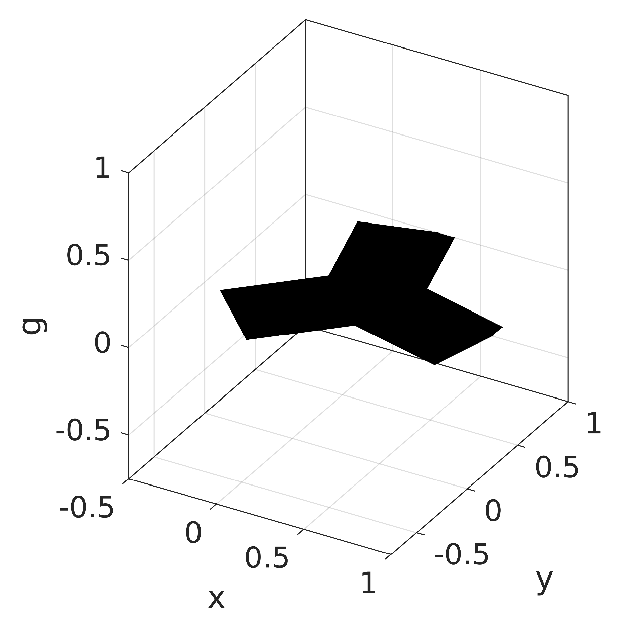
\includegraphics[width=1\linewidth]{./fig/moment_hull_1}
        \caption{}
      \end{subfigure}
      \begin{subfigure}[b]{0.49\textwidth}
        \centering
        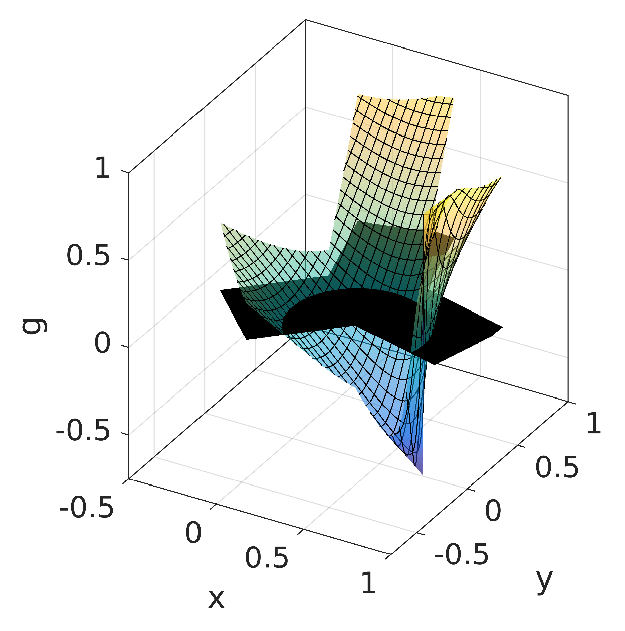
\includegraphics[width=1\linewidth]{fig/moment_hull_2}
        \caption{}
      \end{subfigure}
      \begin{subfigure}[b]{0.49\textwidth}
        \centering
        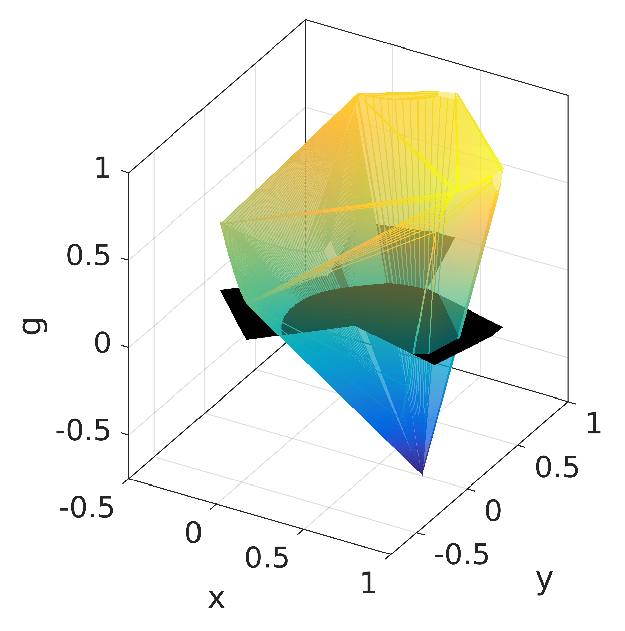
\includegraphics[width=1\linewidth]{fig/moment_hull_3}
        \caption{}
      \end{subfigure}
      \begin{subfigure}[b]{0.49\textwidth}
        \centering
        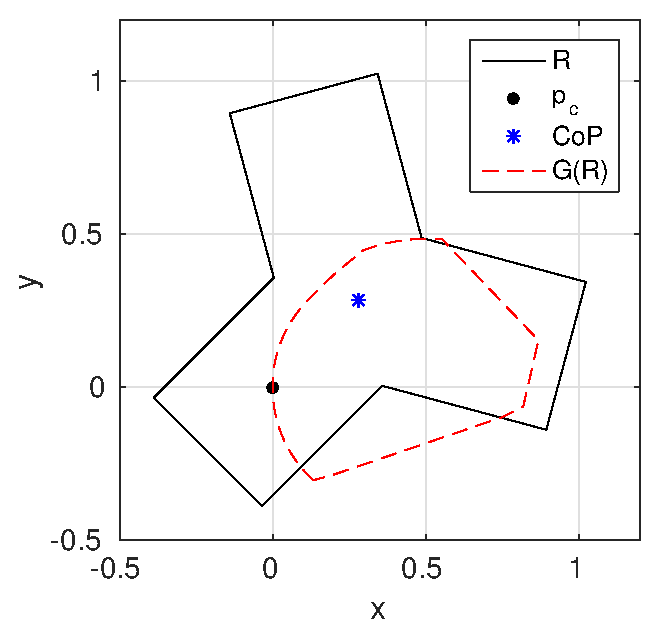
\includegraphics[width=1\linewidth]{fig/CoP_boundary}
        \caption{}
      \end{subfigure}
      % \caption{Example moment envelope for a trigonal 2D object with
      % rotation center $x_{\text{IC}} = 0.75$. (a) Support region
      % $R$. (b) Normalized-moment surface $G(R)$. (c) Convex moment
      % envelope of $G(R)$. (d) Intersection of the moment envelope and
      % the $xy$-plane. The intersection bounds the set of feasible
      % centers of pressure with zero moment.}
      % \label{fig:moment-envelope}
    \end{figure}
  \end{columns}
\end{frame}

\section{Theory}

\begin{frame}{Angular Velocity Bounds Properties}


  \begin{columns}[c,onlytextwidth]
    \column{0.5\textwidth}

    \begin{list}{}{
        \setlength{\leftmargin}{0pt}
        % % \settowidth{\leftmargini}{\usebeamertemplate{itemize item}}
        % % \addtolength{\leftmargini}{\labelsep}
        \setlength{\labelwidth}{0pt}
        \setlength{\labelsep}{0pt}
        % \setlength{\labelindent}{0pt}
        % \setlength{\itemindent}{0pt}
        % \setlength{\leftskip}{-\@totalleftmargin}
      }
    \item Fix $\theta$
    \item $\omega$ is \textit{feasible} if
      \begin{equation*}
      \mathbf{m}_f(\omega) = 0
      \end{equation*}
    \item Feasible set:
      \begin{equation*}
      \Omega = \{\omega\; |\; \mathbf{m}_f(\omega) = 0\}
      \end{equation*}
    \end{list}
    \begin{theorem}
      The feasible set $\Omega$ is connected and bounded.
    \end{theorem}

    % Bounds:
    \begin{align*}
      \alpha &= \max \Omega\\
      \beta &= \min \Omega
    \end{align*}

    \column{0.5\textwidth}

    \begin{figure}
      \centering
      \def\iangle{35} % Angle of the inclined plane
      \begin{tikzpicture}[
        scale=0.60, every node/.style={scale=0.75},
        force/.style={>=latex,draw=black,fill=black},
        axis/.style={densely dashed,draw=gray,font=\small},
        ]
        \fill[draw=black,fill=blue!10,thin,rotate=\iangle] (-0.3,-0.5) rectangle (2.3,.5);
        \draw[rotate=\iangle] (1,0) circle[radius=2.4pt] node[cross] {};
        \draw[rotate=\iangle] (1,0) node[above right] {\tiny CoP};
        \draw [rotate=-62.5] (0,0) ++(0,1) arc (90:30:1.0) node[right] {$\theta$};
        \draw [->,rotate=-120] (0,0) ++(0,1) arc (90:30:1.0);
        {[axis,->]
          \draw (-1,0) -- (2.5,0) node[right] {$x$};
          \draw (0,-1.5) -- (0,2.5) node[above] {$y$};
        }
        {[force,->]
          \draw (0,0) -- ++(0,1.5) node[right] {$\mathbf{v}$};
        }
        \fill (0,0) circle [radius=2.pt];
        % \fill (1.2207,0) circle [radius=1.pt] node[below right] {$x_{\text{\tiny IC}}$};

      \end{tikzpicture}
      % \caption{Motion of a press-pulled slider.}
      % \BB{Define variables and provide a short explanation of the figure.}}
      % \label{fig:presspull-motion}
    \end{figure}

    \begin{tikzpicture}
      \node[anchor=south west,inner sep=0] (image) at (0,0) {\includegraphics[width=\linewidth]{fig/omega_bounds_1}};
      \draw[line width=1.25] (2.3,2.34) -- ++(0,1.08) node[right] {$\Omega$};
      \definecolor{BLUE}{RGB}{0,113,188}
      \definecolor{ORANGE}{RGB}{216,82,24}
      \draw[line width=1.25,color=BLUE] (1.75,1.5) -- ++(0.25,0) node[right] {$\beta$};
      \draw[line width=1.25,color=ORANGE] (3.375,2.775) -- ++(0.25,0) node[right] {$\alpha$};
    \end{tikzpicture}

  \end{columns}
\end{frame}

\begin{frame}{Orientation Bounds}
    \begin{columns}[c,onlytextwidth]
    \column{0.5\textwidth}

    \begin{list}{}{
        \setlength{\leftmargin}{0pt}
        % % \settowidth{\leftmargini}{\usebeamertemplate{itemize item}}
        % % \addtolength{\leftmargini}{\labelsep}
        \setlength{\labelwidth}{0pt}
        \setlength{\labelsep}{0pt}
        % \setlength{\labelindent}{0pt}
        % \setlength{\itemindent}{0pt}
        % \setlength{\leftskip}{-\@totalleftmargin}
      }
    \item Contact point path:\vspace{-2mm}
      \begin{align*}
        &\gamma : \mathbb{R}\rightarrow\mathbb{R}^2, \quad \lVert\dot{\gamma}\rVert = 1\\
        &\rho = \tan^{-1}(\dot{\gamma}_y,\dot{\gamma}_x)
      \end{align*}
    \item Dynamics:\vspace{-2mm}
      \begin{align*}
        &\left.
        \begin{aligned}
          \dot{x} &= \cos(\rho)\\
          \dot{y} &= \sin(\rho)\\
          \dot{\varphi} &= \omega(\varphi - \rho + \pi)
        \end{aligned}\quad\right\}\quad\text{state}\\
        &\left.
        \begin{aligned}
        \dot{u} &=  \alpha(u - \rho + \pi) \\
        \dot{\ell} &=  \beta(\ell - \rho + \pi)
        \end{aligned}\quad\:\right\}\quad\text{bounds}
      \end{align*}
    \end{list}\vspace{-3mm}
    \begin{theorem}
      Given $\gamma$ and $\ell_0=\varphi_0=u_0$, then
      $\ell(t) \leq \varphi(t) \leq u(t), t \in [0,\infty)$
    \end{theorem}

    \column{0.5\textwidth}

    \begin{figure}
      \centering
      \def\iangle{-115} % Angle of the inclined plane
      \begin{tikzpicture}[
        scale=0.80, every node/.style={scale=0.75},
        force/.style={>=latex,draw=black,fill=black},
        axis/.style={densely dashed,draw=gray,font=\small},
        ]
        \fill[draw=black,fill=blue!10,thin,rotate=\iangle] (-0.3,-0.5) rectangle (2.3,.5);
        \draw[rotate=\iangle] (1,0) circle[radius=2.4pt] node[cross] {};
        \draw[rotate=\iangle] (1,0) node[below left] {\tiny CoP};

        % rho
        \def\rhol{0.50}
        \draw [rotate=0] (0,0) -- ++(\rhol,0) arc (0:130:\rhol) -- (0,0);
        \draw [dotted,rotate=0] (0,0) ++(\rhol,0) arc (0:50:\rhol) node[above right] {$\rho$};
        % varphi
        \def\phil{0.75}
        \draw [rotate=0] (0,0) -- ++(\phil,0) arc (0:-115:\phil) -- (0,0);
        \draw [rotate=0] (0,0) ++(\phil,0) arc (0:-30:\phil) node[right] {$\varphi$};
        % varphi - rho + pi
        \def\vrpl{1.}
        \draw [rotate=-50] (0,0) -- ++(\vrpl,0) arc (0:-65:\vrpl) -- (0,0);
        \draw [rotate=-50] (0,0) -- ++(\vrpl,0) arc (0:-30:\vrpl) node[below right] {$\varphi-\rho+\pi$};
        {[force,->]
          \draw[rotate=40] (0,0) -- ++(0,1.5) node[right] {$\dot{\gamma}$};
        }
        \fill (0,0) circle [radius=2.pt] node[left] {$(x,y)$};
        % \fill (1.2207,0) circle [radius=1.pt] node[below right] {$x_{\text{\tiny IC}}$};

      \end{tikzpicture}
      % \caption{Motion of a press-pulled slider.}
      % \BB{Define variables and provide a short explanation of the figure.}}
      % \label{fig:presspull-motion}
    \end{figure}

    \begin{tikzpicture}
      \node[anchor=south west,inner sep=0] (image) at (0,0) {\includegraphics[width=\linewidth]{fig/omega_bounds_1}};
      % \draw[line width=1.25] (2.3,2.34) -- ++(0,1.08) node[right] {$\Omega$};
      \definecolor{BLUE}{RGB}{0,113,188}
      \definecolor{ORANGE}{RGB}{216,82,24}
      \draw[line width=1.25,color=BLUE] (1.75,1.5) -- ++(0.25,0) node[right] {$\beta$};
      \draw[line width=1.25,color=ORANGE] (3.375,2.775) -- ++(0.25,0) node[right] {$\alpha$};
    \end{tikzpicture}

  \end{columns}
\end{frame}

\section{Methods}

\begin{frame}{Exact Angular Velocity Bounds}
\end{frame}

\begin{frame}{Planning for Robotic Pulling}
\end{frame}

\section{Experiments}

\begin{frame}{Robotic Pulling}
  
\end{frame}

% \begin{frame}[fragile]{Metropolis}

%   The \themename theme is a Beamer theme with minimal visual noise
%   inspired by the \href{https://github.com/hsrmbeamertheme/hsrmbeamertheme}{\textsc{hsrm} Beamer
%   Theme} by Benjamin Weiss.

%   Enable the theme by loading

%   \begin{verbatim}    \documentclass{beamer}
%     \usetheme{metropolis}\end{verbatim}

%   Note, that you have to have Mozilla's \emph{Fira Sans} font and XeTeX
%   installed to enjoy this wonderful typography.
% \end{frame}
% \begin{frame}[fragile]{Sections}
%   Sections group slides of the same topic

%   \begin{verbatim}    \section{Elements}\end{verbatim}

%   for which \themename provides a nice progress indicator \ldots
% \end{frame}

% \section{Titleformats}

% \begin{frame}{Metropolis titleformats}
% 	\themename supports 4 different titleformats:
% 	\begin{itemize}
% 		\item Regular
% 		\item \textsc{Smallcaps}
% 		\item \textsc{allsmallcaps}
% 		\item ALLCAPS
% 	\end{itemize}
% 	They can either be set at once for every title type or individually.
% \end{frame}

% {
%     \metroset{titleformat frame=smallcaps}
% \begin{frame}{Small caps}
% 	This frame uses the \texttt{smallcaps} titleformat.

% 	\begin{alertblock}{Potential Problems}
% 		Be aware, that not every font supports small caps. If for example you typeset your presentation with pdfTeX and the Computer Modern Sans Serif font, every text in smallcaps will be typeset with the Computer Modern Serif font instead.
% 	\end{alertblock}
% \end{frame}
% }

% {
% \metroset{titleformat frame=allsmallcaps}
% \begin{frame}{All small caps}
% 	This frame uses the \texttt{allsmallcaps} titleformat.

% 	\begin{alertblock}{Potential problems}
% 		As this titleformat also uses smallcaps you face the same problems as with the \texttt{smallcaps} titleformat. Additionally this format can cause some other problems. Please refer to the documentation if you consider using it.

% 		As a rule of thumb: Just use it for plaintext-only titles.
% 	\end{alertblock}
% \end{frame}
% }

% {
% \metroset{titleformat frame=allcaps}
% \begin{frame}{All caps}
% 	This frame uses the \texttt{allcaps} titleformat.

% 	\begin{alertblock}{Potential Problems}
% 		This titleformat is not as problematic as the \texttt{allsmallcaps} format, but basically suffers from the same deficiencies. So please have a look at the documentation if you want to use it.
% 	\end{alertblock}
% \end{frame}
% }

% \section{Elements}

% \begin{frame}[fragile]{Typography}
%       \begin{verbatim}The theme provides sensible defaults to
% \emph{emphasize} text, \alert{accent} parts
% or show \textbf{bold} results.\end{verbatim}

%   \begin{center}becomes\end{center}

%   The theme provides sensible defaults to \emph{emphasize} text,
%   \alert{accent} parts or show \textbf{bold} results.
% \end{frame}

% \begin{frame}{Font feature test}
%   \begin{itemize}
%     \item Regular
%     \item \textit{Italic}
%     \item \textsc{SmallCaps}
%     \item \textbf{Bold}
%     \item \textbf{\textit{Bold Italic}}
%     \item \textbf{\textsc{Bold SmallCaps}}
%     \item \texttt{Monospace}
%     \item \texttt{\textit{Monospace Italic}}
%     \item \texttt{\textbf{Monospace Bold}}
%     \item \texttt{\textbf{\textit{Monospace Bold Italic}}}
%   \end{itemize}
% \end{frame}

% \begin{frame}{Lists}
%   \begin{columns}[T,onlytextwidth]
%     \column{0.33\textwidth}
%       Items
%       \begin{itemize}
%         \item Milk \item Eggs \item Potatos
%       \end{itemize}

%     \column{0.33\textwidth}
%       Enumerations
%       \begin{enumerate}
%         \item First, \item Second and \item Last.
%       \end{enumerate}

%     \column{0.33\textwidth}
%       Descriptions
%       \begin{description}
%         \item[PowerPoint] Meeh. \item[Beamer] Yeeeha.
%       \end{description}
%   \end{columns}
% \end{frame}
% \begin{frame}{Animation}
%   \begin{itemize}[<+- | alert@+>]
%     \item \alert<4>{This is\only<4>{ really} important}
%     \item Now this
%     \item And now this
%   \end{itemize}
% \end{frame}
% \begin{frame}{Figures}
%   \begin{figure}
%     \newcounter{density}
%     \setcounter{density}{20}
%     \begin{tikzpicture}
%       \def\couleur{alerted text.fg}
%       \path[coordinate] (0,0)  coordinate(A)
%                   ++( 90:5cm) coordinate(B)
%                   ++(0:5cm) coordinate(C)
%                   ++(-90:5cm) coordinate(D);
%       \draw[fill=\couleur!\thedensity] (A) -- (B) -- (C) --(D) -- cycle;
%       \foreach \x in {1,...,40}{%
%           \pgfmathsetcounter{density}{\thedensity+20}
%           \setcounter{density}{\thedensity}
%           \path[coordinate] coordinate(X) at (A){};
%           \path[coordinate] (A) -- (B) coordinate[pos=.10](A)
%                               -- (C) coordinate[pos=.10](B)
%                               -- (D) coordinate[pos=.10](C)
%                               -- (X) coordinate[pos=.10](D);
%           \draw[fill=\couleur!\thedensity] (A)--(B)--(C)-- (D) -- cycle;
%       }
%     \end{tikzpicture}
%     \caption{Rotated square from
%     \href{http://www.texample.net/tikz/examples/rotated-polygons/}{texample.net}.}
%   \end{figure}
% \end{frame}
% \begin{frame}{Tables}
%   \begin{table}
%     \caption{Largest cities in the world (source: Wikipedia)}
%     \begin{tabular}{@{} lr @{}}
%       \toprule
%       City & Population\\
%       \midrule
%       Mexico City & 20,116,842\\
%       Shanghai & 19,210,000\\
%       Peking & 15,796,450\\
%       Istanbul & 14,160,467\\
%       \bottomrule
%     \end{tabular}
%   \end{table}
% \end{frame}
% \begin{frame}{Blocks}
%   Three different block environments are pre-defined and may be styled with an
%   optional background color.

%   \begin{columns}[T,onlytextwidth]
%     \column{0.5\textwidth}
%       \begin{block}{Default}
%         Block content.
%       \end{block}

%       \begin{alertblock}{Alert}
%         Block content.
%       \end{alertblock}

%       \begin{exampleblock}{Example}
%         Block content.
%       \end{exampleblock}

%     \column{0.5\textwidth}

%       \metroset{block=fill}

%       \begin{block}{Default}
%         Block content.
%       \end{block}

%       \begin{alertblock}{Alert}
%         Block content.
%       \end{alertblock}

%       \begin{exampleblock}{Example}
%         Block content.
%       \end{exampleblock}

%   \end{columns}
% \end{frame}
% \begin{frame}{Math}
%   \begin{equation*}
%     e = \lim_{n\to \infty} \left(1 + \frac{1}{n}\right)^n
%   \end{equation*}
% \end{frame}
% \begin{frame}{Line plots}
%   \begin{figure}
%     \begin{tikzpicture}
%       \begin{axis}[
%         mlineplot,
%         width=0.9\textwidth,
%         height=6cm,
%       ]

%         \addplot {sin(deg(x))};
%         \addplot+[samples=100] {sin(deg(2*x))};

%       \end{axis}
%     \end{tikzpicture}
%   \end{figure}
% \end{frame}
% \begin{frame}{Bar charts}
%   \begin{figure}
%     \begin{tikzpicture}
%       \begin{axis}[
%         mbarplot,
%         xlabel={Foo},
%         ylabel={Bar},
%         width=0.9\textwidth,
%         height=6cm,
%       ]

%       \addplot plot coordinates {(1, 20) (2, 25) (3, 22.4) (4, 12.4)};
%       \addplot plot coordinates {(1, 18) (2, 24) (3, 23.5) (4, 13.2)};
%       \addplot plot coordinates {(1, 10) (2, 19) (3, 25) (4, 15.2)};

%       \legend{lorem, ipsum, dolor}

%       \end{axis}
%     \end{tikzpicture}
%   \end{figure}
% \end{frame}
% \begin{frame}{Quotes}
%   \begin{quote}
%     Veni, Vidi, Vici
%   \end{quote}
% \end{frame}

% {%
% \setbeamertemplate{frame footer}{My custom footer}
% \begin{frame}[fragile]{Frame footer}
%     \themename defines a custom beamer template to add a text to the footer. It can be set via
%     \begin{verbatim}\setbeamertemplate{frame footer}{My custom footer}\end{verbatim}
% \end{frame}
% }

% \begin{frame}{References}
%   Some references to showcase [allowframebreaks] \cite{Mason,ConcreteMath,Simpson,Er01,greenwade93}
% \end{frame}

\section{Conclusion}

\begin{frame}{Summary}

  Get the source of this theme and the demo presentation from

  \begin{center}\url{github.com/matze/mtheme}\end{center}

  The theme \emph{itself} is licensed under a
  \href{http://creativecommons.org/licenses/by-sa/4.0/}{Creative Commons
  Attribution-ShareAlike 4.0 International License}.

  \begin{center}\ccbysa\end{center}

\end{frame}

\begin{frame}[standout]
  Questions?
\end{frame}

\appendix

\begin{frame}[fragile]{Backup slides}
  Sometimes, it is useful to add slides at the end of your presentation to
  refer to during audience questions.

  The best way to do this is to include the \verb|appendixnumberbeamer|
  package in your preamble and call \verb|\appendix| before your backup slides.

  \themename will automatically turn off slide numbering and progress bars for
  slides in the appendix.
\end{frame}

\begin{frame}[allowframebreaks]{References}

  \bibliography{references}
  \bibliographystyle{abbrv}

\end{frame}

\end{document}
